\chapter{Experimental Testing}

\section{Virtual Spring-damper Tests}
$r_0 = 0.3\ m$\\
$r_{offset} = r - r_0 = 0.13\ m$

\begin{figure}
\centering
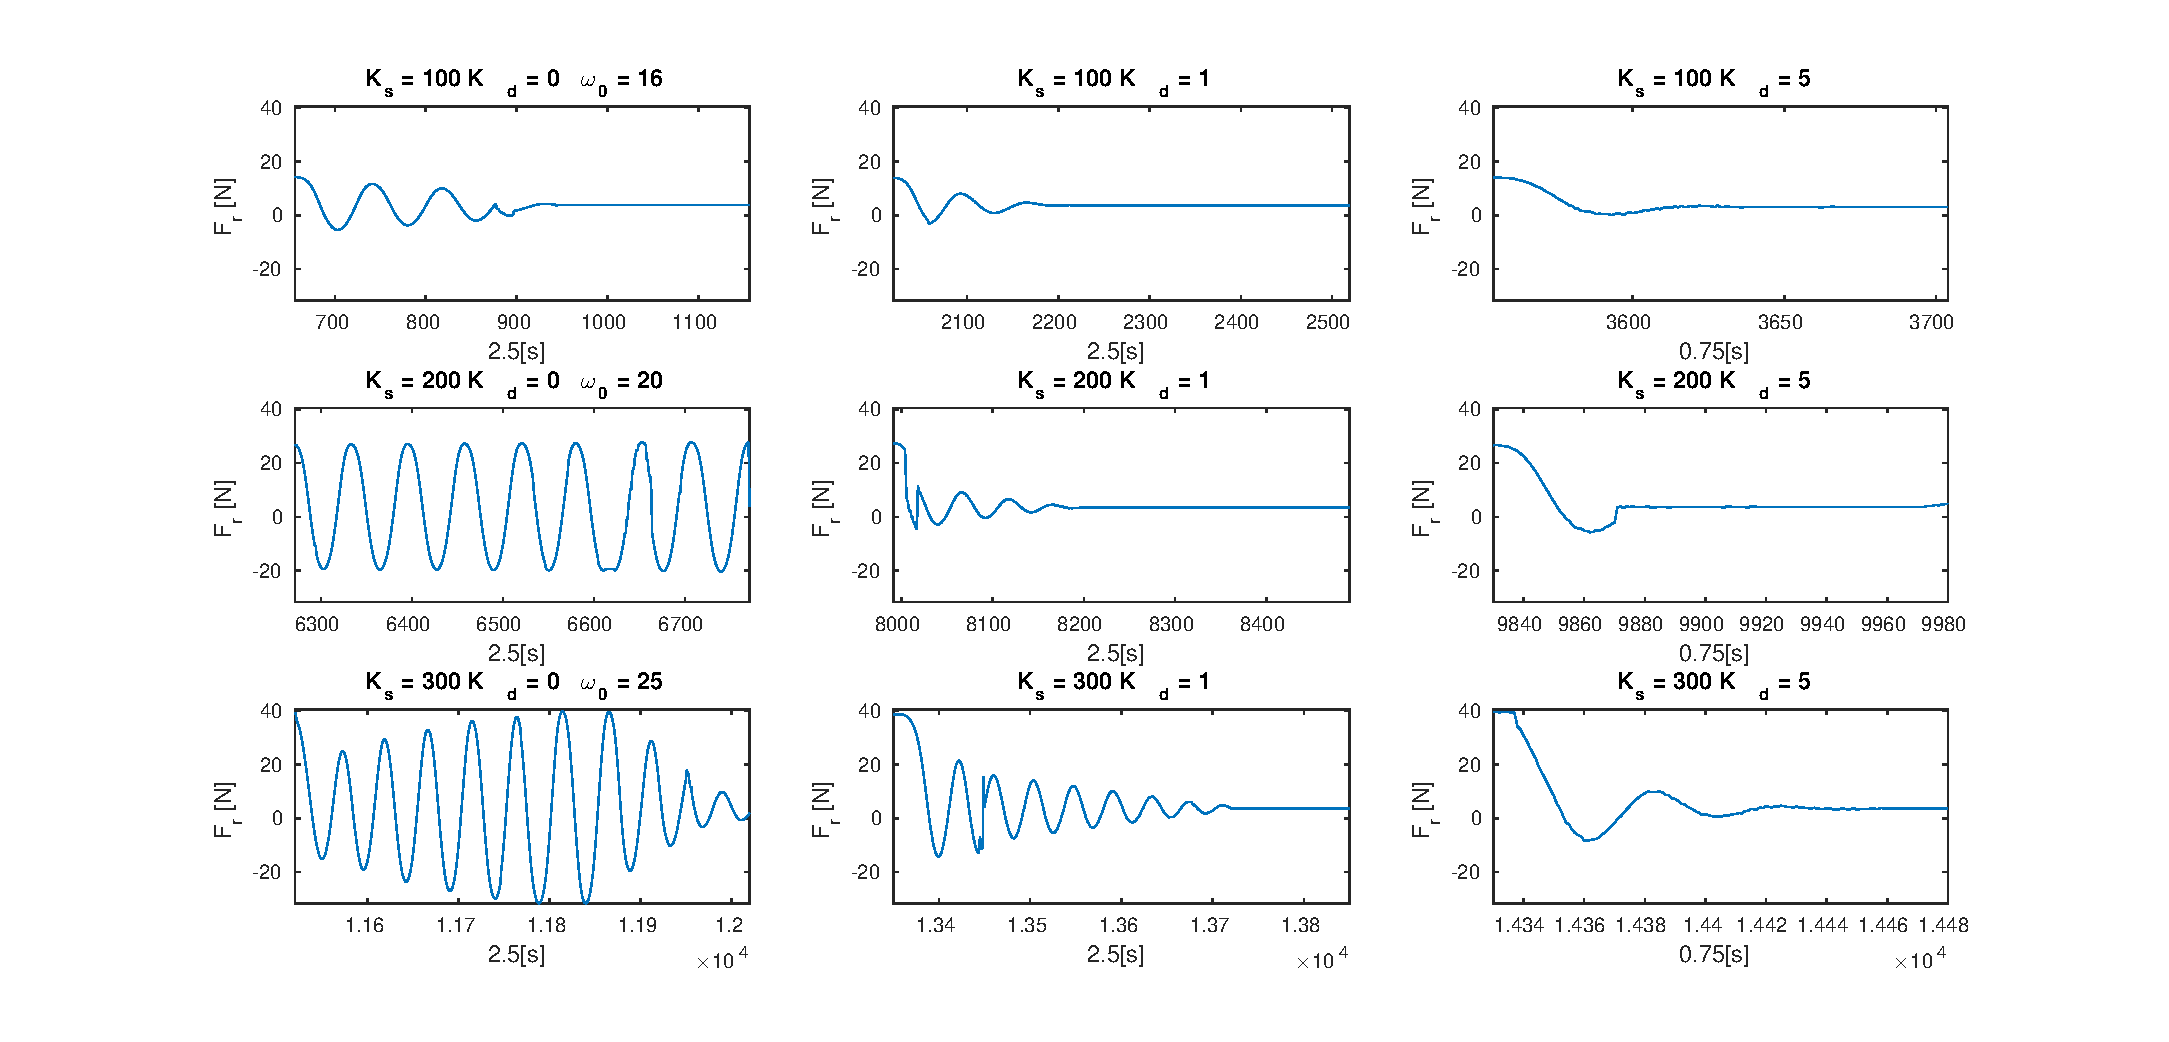
\includegraphics[width=1\textwidth]{images/experiments/spring-damper-tests.eps} 
\caption{Leg spring damper testing for radial offset.}
\label{fig:spring-damper-tests}
\end{figure}

\section{Drop Tests}

\begin{figure}
\centering
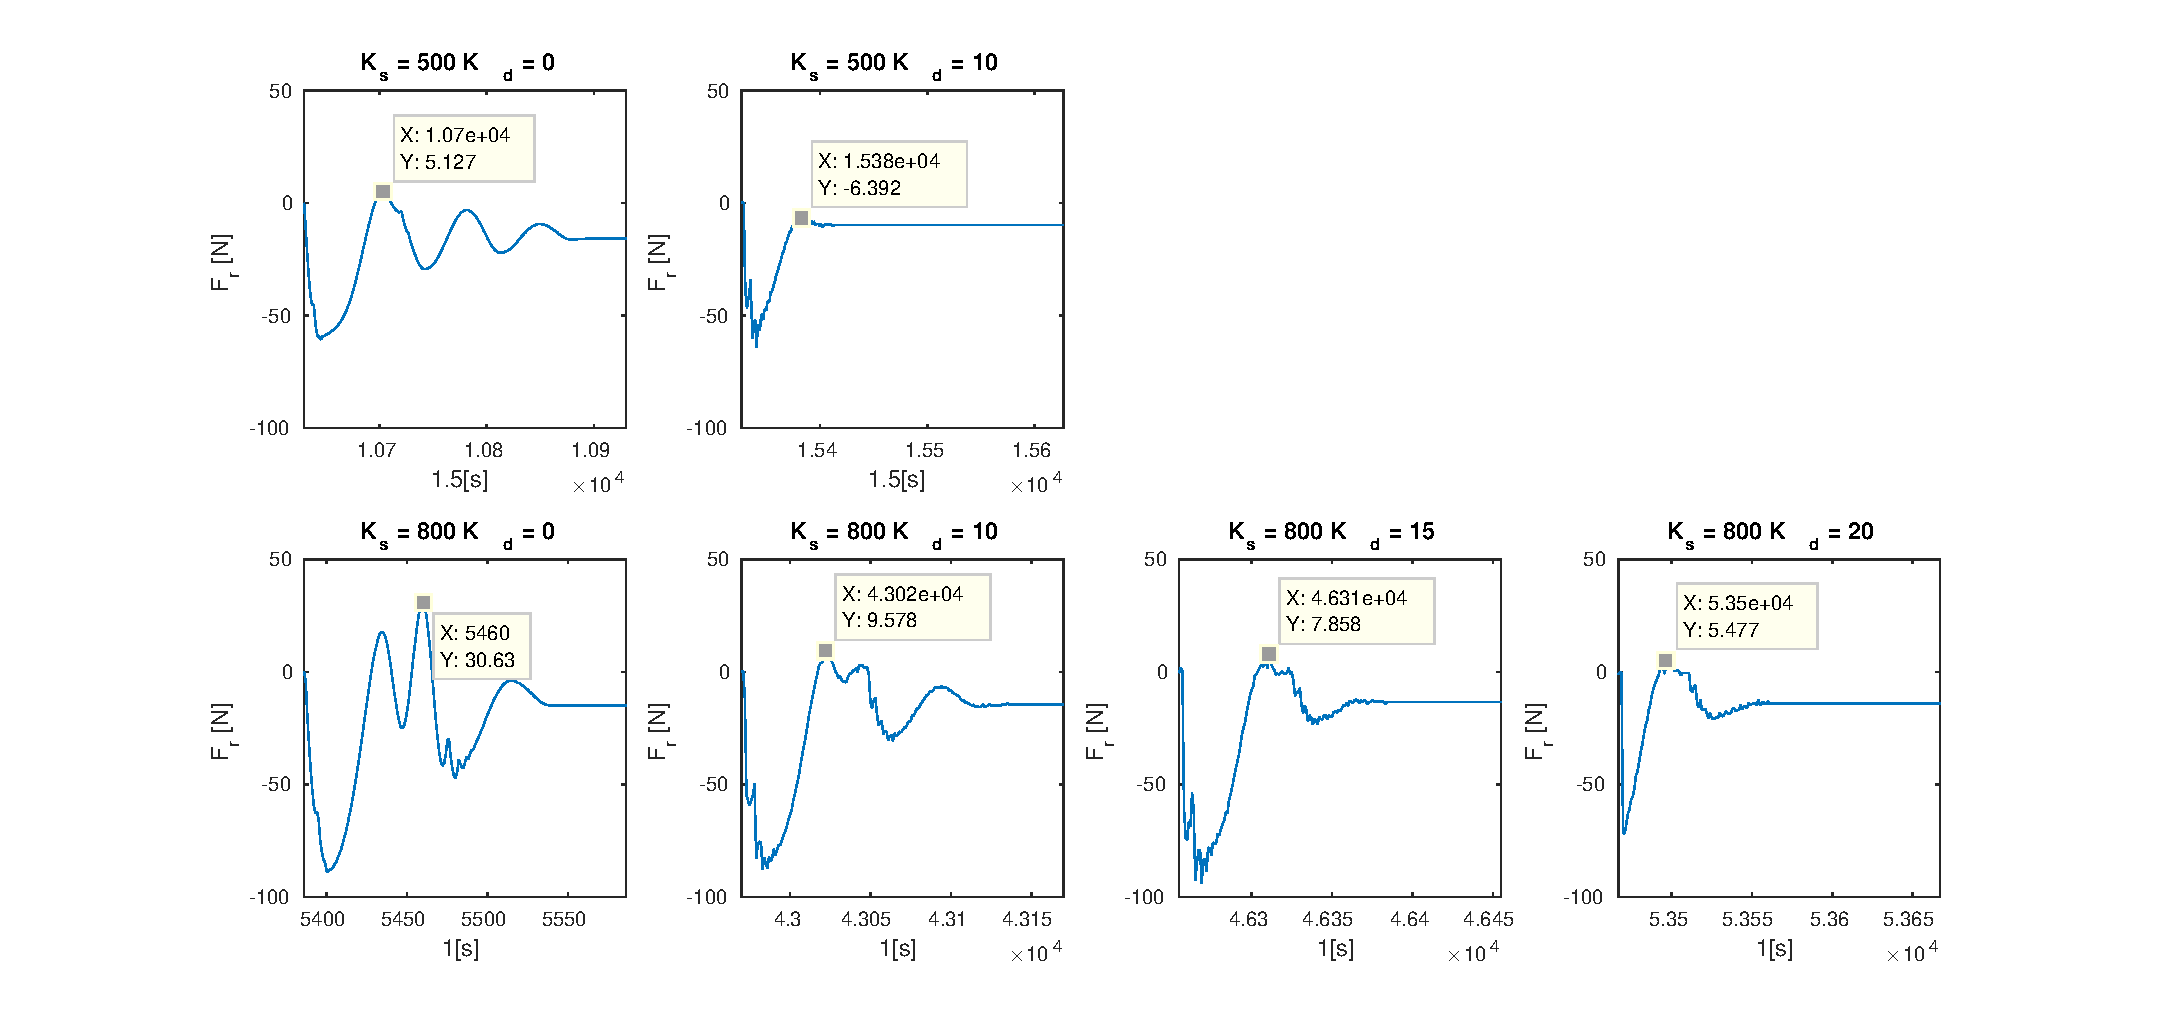
\includegraphics[width=1\textwidth]{images/experiments/drop-test-force-plots.eps} 
\caption{Leg spring damper drop testing.}
\label{fig:drop-tests}
\end{figure}

\section{Launch Tests}

\begin{figure}
\centering
\subfloat[][Frame 1.]{
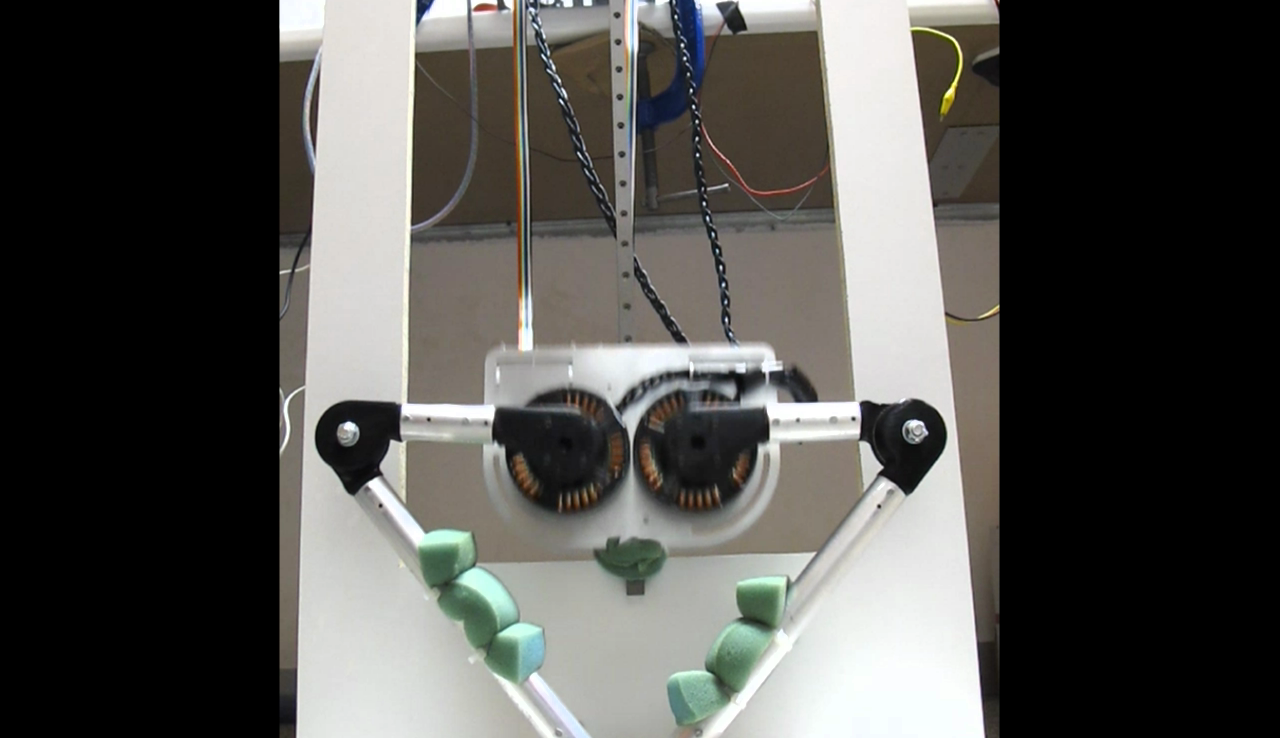
\includegraphics[width=0.4\textwidth]{images/experiments/jump/1.png} 
}
\subfloat[][Frame 2.]{
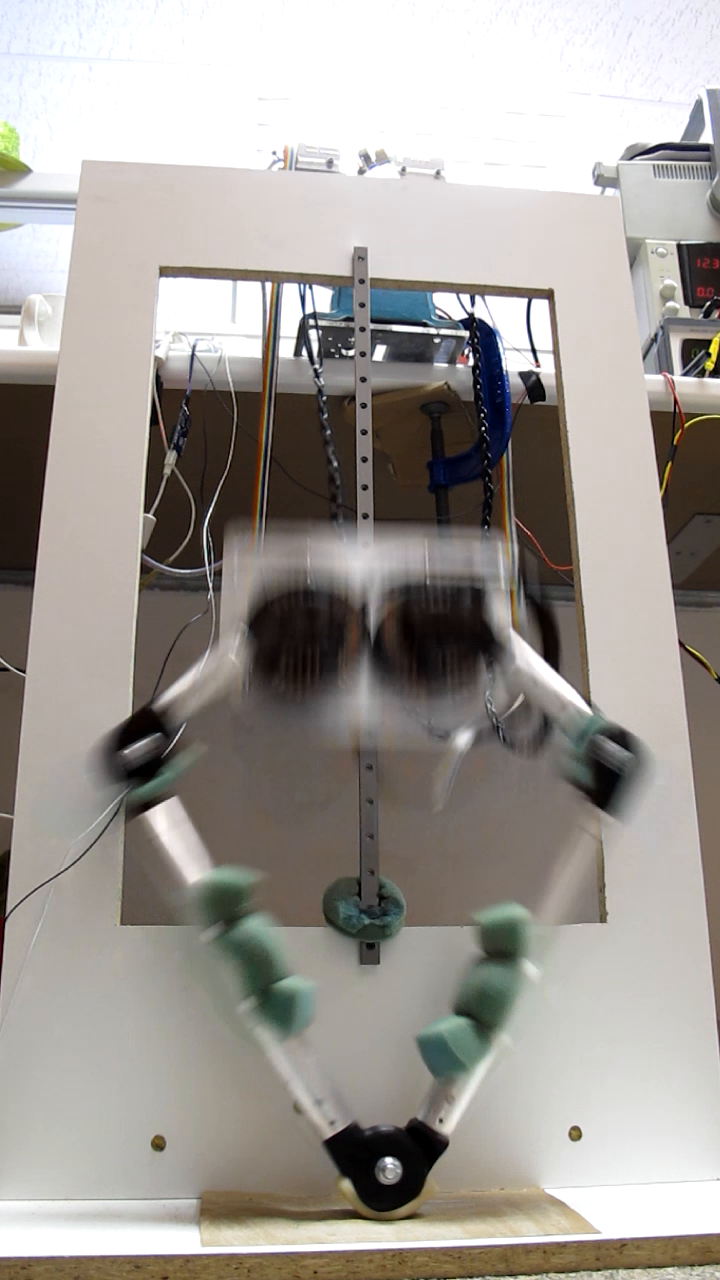
\includegraphics[width=0.4\textwidth]{images/experiments/jump/2.png} 
}

\subfloat[][Frame 3.]{
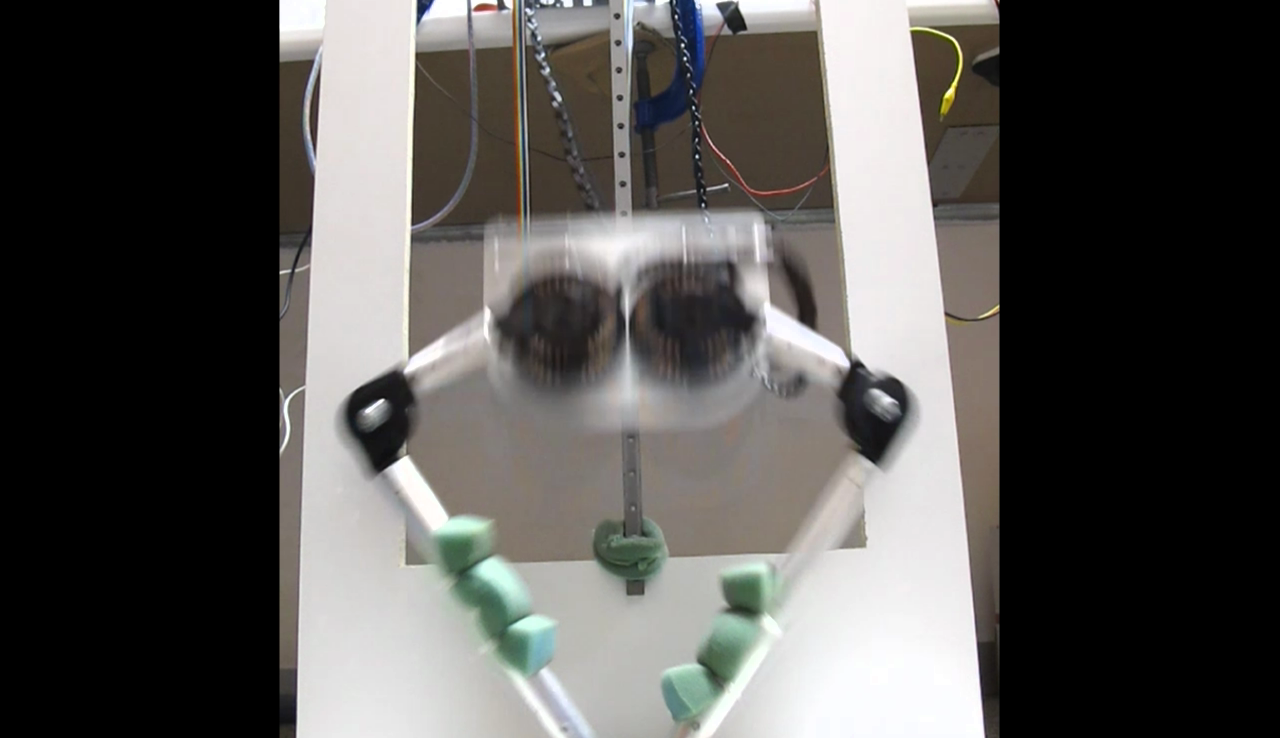
\includegraphics[width=0.4\textwidth]{images/experiments/jump/3.png} 
}
\subfloat[][Frame 4.]{
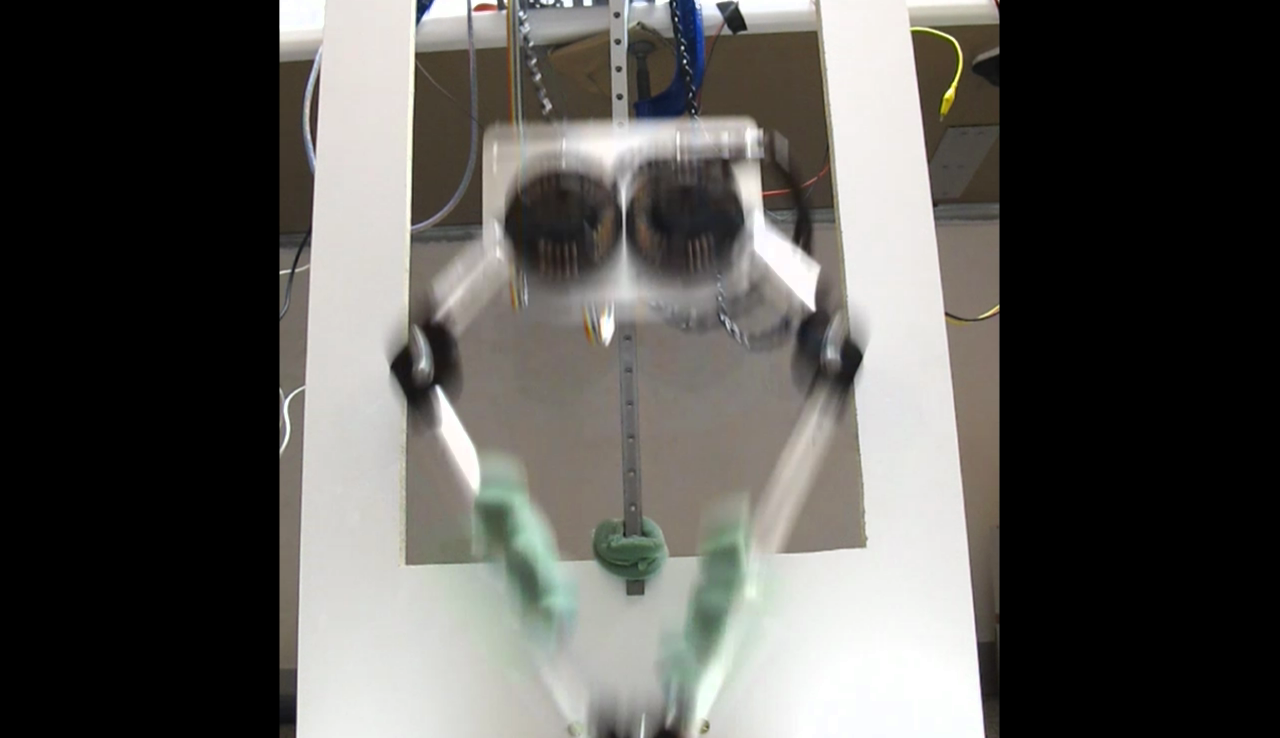
\includegraphics[width=0.4\textwidth]{images/experiments/jump/4.png} 
}

\subfloat[][Frame 5.]{
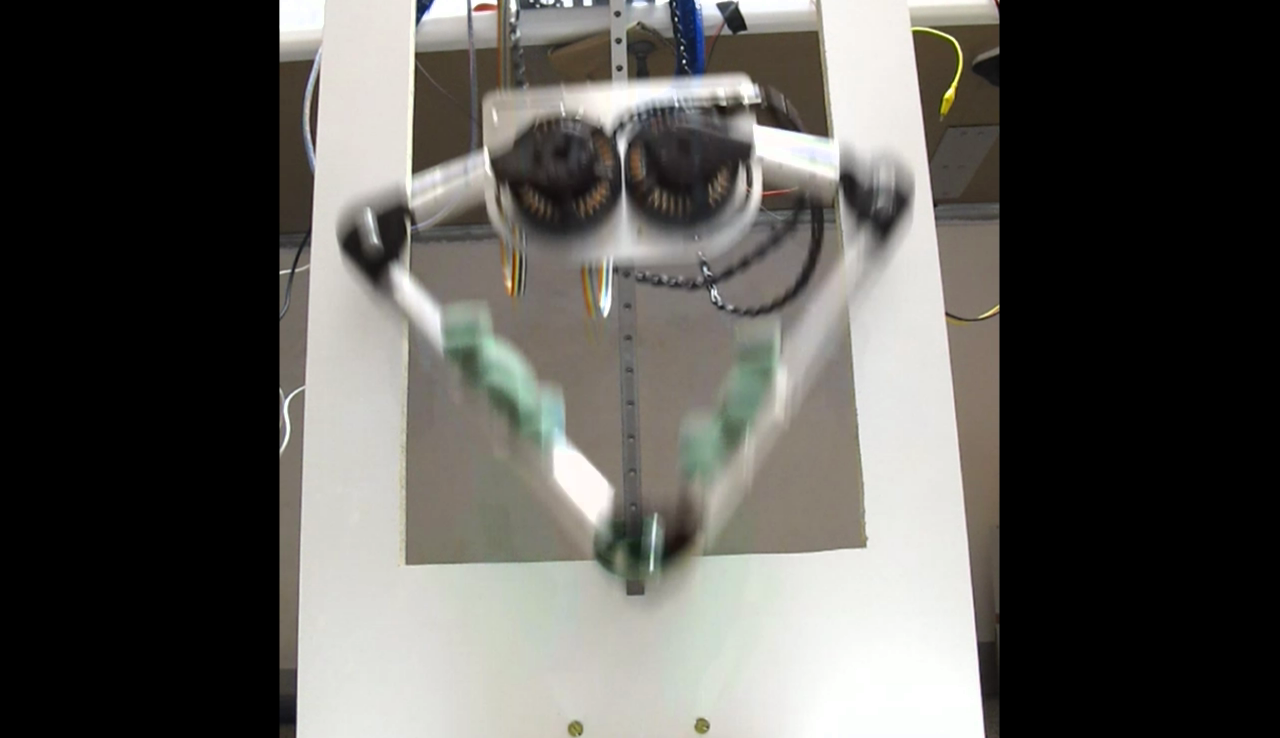
\includegraphics[width=0.4\textwidth]{images/experiments/jump/5.png} 
}
\subfloat[][Frame 6.]{
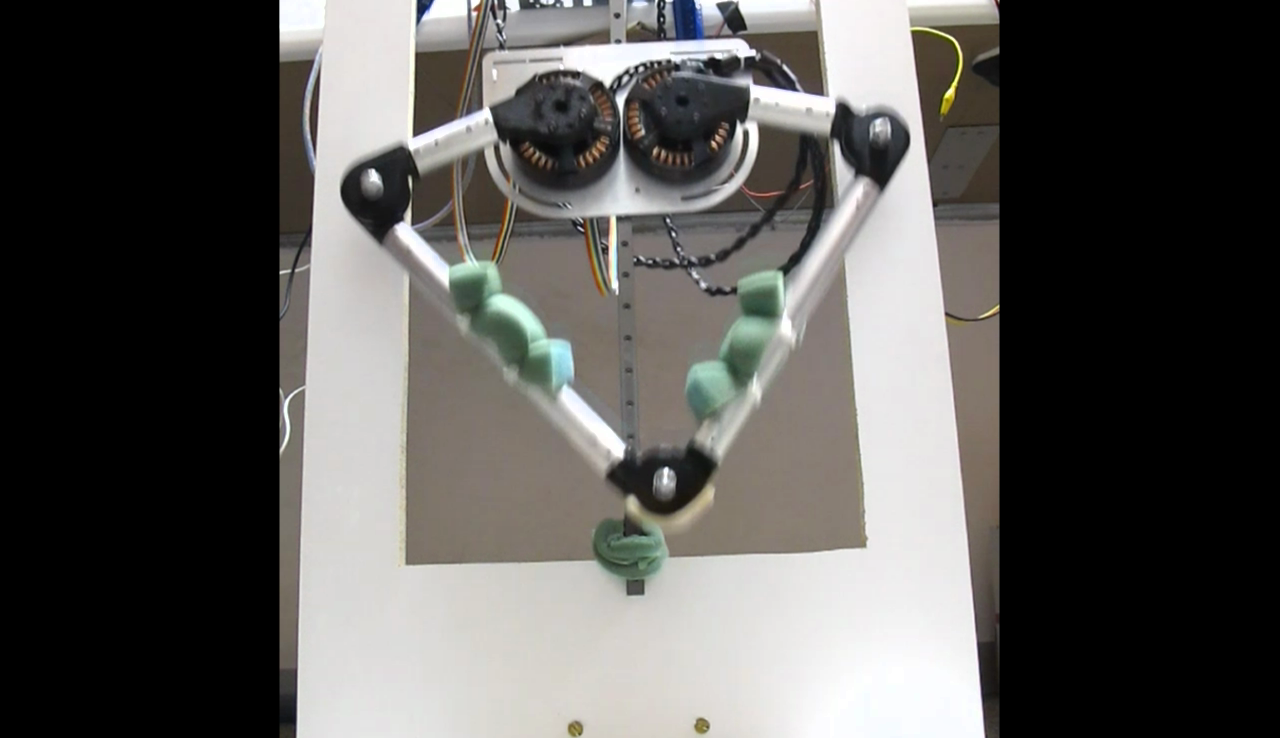
\includegraphics[width=0.4\textwidth]{images/experiments/jump/6.png} 
}

\subfloat[][Frame 7.]{
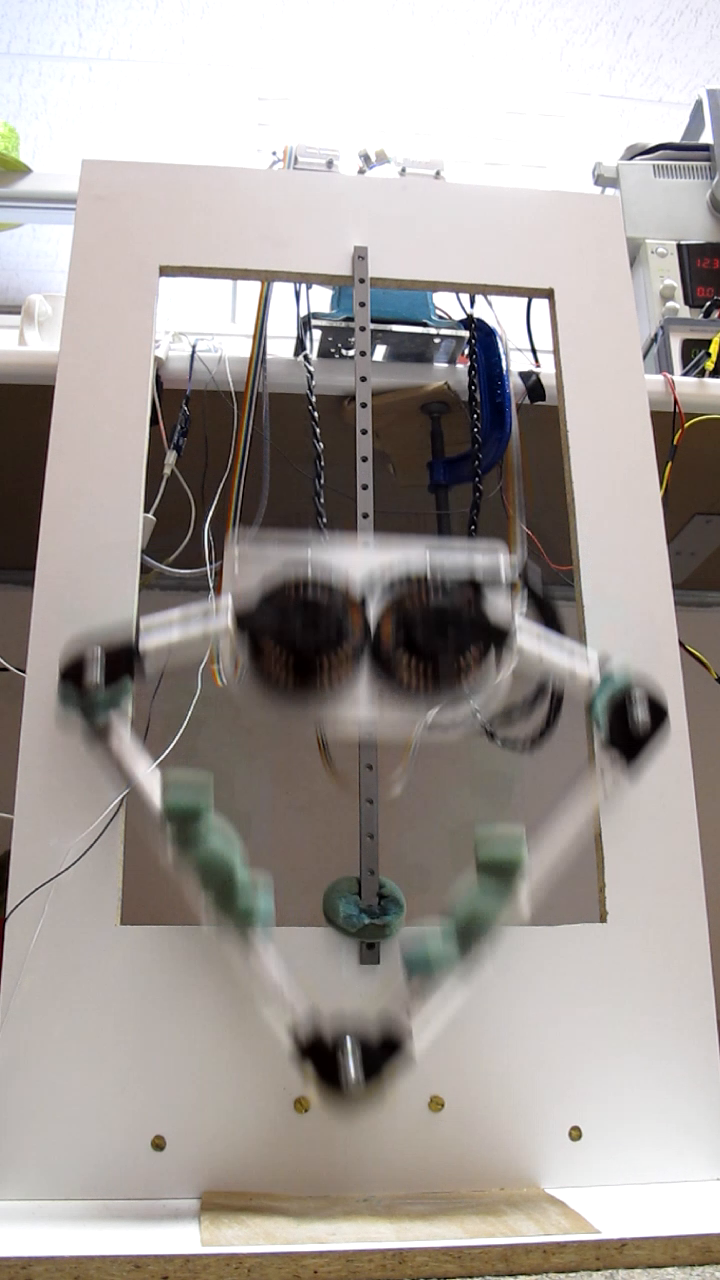
\includegraphics[width=0.4\textwidth]{images/experiments/jump/7.png} 
}
\subfloat[][Frame 8.]{
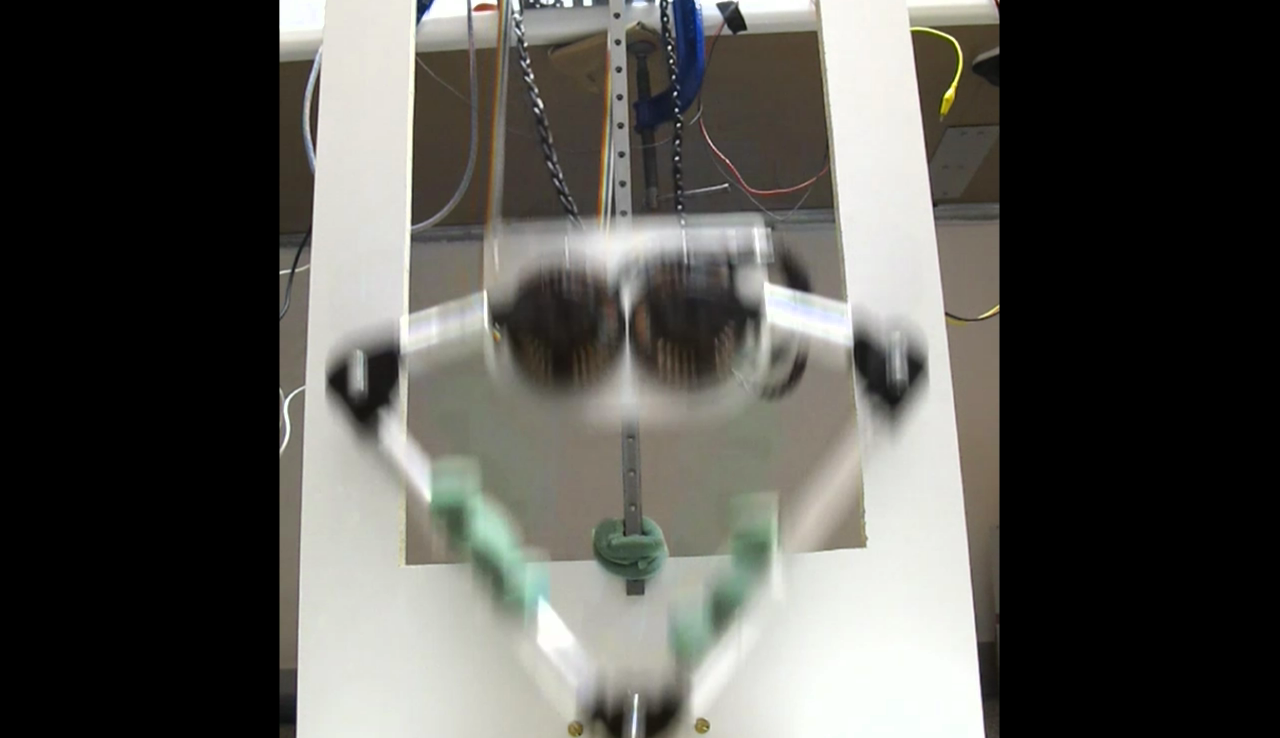
\includegraphics[width=0.4\textwidth]{images/experiments/jump/8.png} 
}

\subfloat[][Frame 9.]{
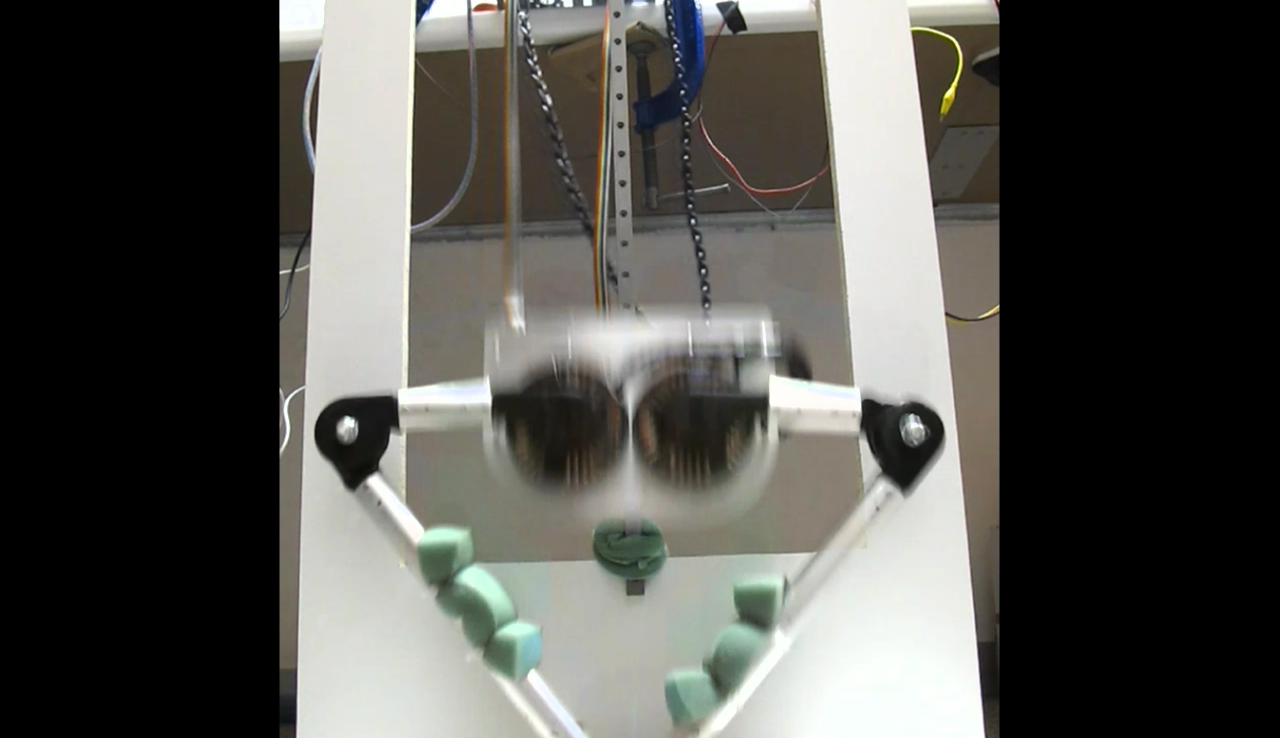
\includegraphics[width=0.4\textwidth]{images/experiments/jump/9.png} 
}
\subfloat[][Frame 10.]{
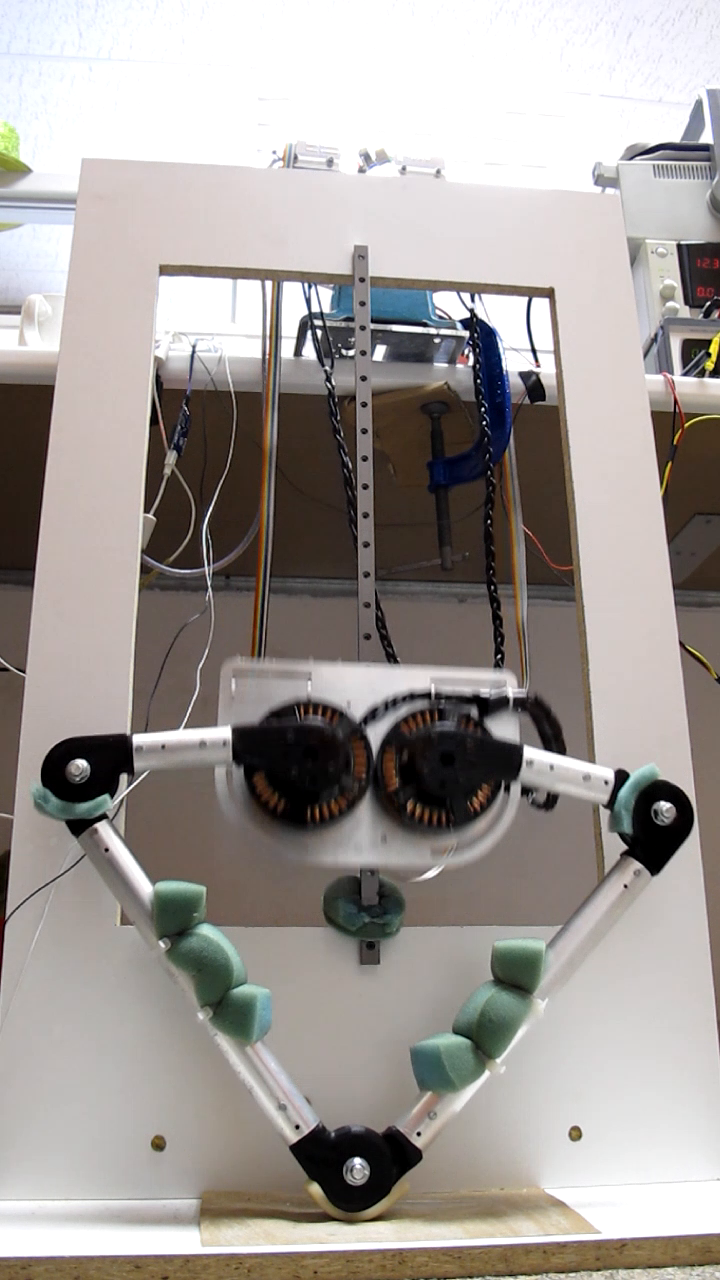
\includegraphics[width=0.4\textwidth]{images/experiments/jump/10.png} 
}
\caption{Leg launch with compliant landing.}
\end{figure}

